\documentclass[a4paper,10pt]{article}
\usepackage[utf8]{inputenc}
\usepackage[english]{babel}
\usepackage{float}
\usepackage{graphicx}
\usepackage{caption}
\usepackage{subcaption}
\usepackage{amsmath}
\usepackage{multirow}

%opening
\title{Deep convolutional networks for protein fold quality assessment}
\author{}

\begin{document}

\maketitle

\begin{abstract}

\end{abstract}

\section{Introduction}
% % Some of this will have to be adapted to the readership of Proteins
% (It's sometimes a bit too elementary.)


The protein folding problem \cite{dill2012folding} remains one of the
outstanding challenges in structural biology. While it is usually
defined as the task of predicting the three-dimensional (3D) structure
of a protein from its amino acid sequence, it can be cast as a ranking
problem: Given a number of structural models of various quality, can
we computationally predict how close each of these models is to the
native fold of the protein?

Progress in the field is monitored through the Critical Assessment of
protein Structure Prediction (CASP) competition \cite{moult1995large},
a community-wide experiment to evaluate the accuracy of protein
folding methods at predicting protein structures ahead of their
publication. Most methods participating in the competition include a
conformational sampling step, which generates a number of plausible
protein conformations, and a quality assessment (QA) step, which
attempts to select those conformations closest to the unknown native
structure.

In this paper we explore the application of deep learning to the
problem of protein decoys quality assessment. Deep learning (DL) has
recently garnered considerable interest in the research
community \cite{lecun2015deep}, particularly in computer vision and
image recognition. Unlike more ``shallow'' machine learning
approaches, DL improves model performance by learning a hierarchical
representation of the data at hand. It alleviates the need for feature
engineering, which has traditionally constituted the bulk of the work
done by researchers.

DL has recently been applied to biological data and has yielded
remarkable results for predicting the effects of genetic variations on
human RNA splicing \cite{xiong2015human}, for identifying DNA- and
RNA-binding motifs \cite{alipanahi2015predicting}, and for predicting
the effects of non-coding DNA variants with single nucleotide
precision \cite{zhou2015predicting}. These successes have one thing in
common: they use raw data directly as input and do not attempt to
engineer features from them.

\subsection{Related work}
Deep learning methods have also been applied in the field of protein
structure quality assessment \cite{nguyen2014dlpro, cao2016deepqa,
uziela2017proq3d}. For instance, DeepQA \cite{cao2016deepqa} uses 9
scores from other QA models and 7 physico-chemical features extracted
from the structure as input features to a deep Boltzmann
machine \cite{}. In the DL-PRO algorithm \cite{nguyen2014dlpro},
authors first compute contact maps of the decoys and compress them
using PCA. The vectors from PCA are then fed into an autoencoder to
predict the score of the decoy. The authors that apply the deep
learning methods use them as the ordinary 'shallow' classifiers.
Therefore they do not get all the advantages these new techniques
offer.

More in line with the ``end-to-end'' spirit of deep learning, methods
using as input a 3D representation of the structure have been
developed to score protein-ligand
poses \cite{ragoza2017ligandscoring}, to predict ligand-binding
protein pockets \cite{jimenez2017deepsite}, or to predict the effect
of a mutation \cite{torng2017}.
% Say something about what is bad and what is good about them.



\section{Materials and Methods}

\subsection{Datasets}
% 
We train and assess our method using the protein decoy datasets from
the CASP competition \cite{moult2014critical}.  We use the CASP7 to
CASP10 data as training set and the CASP11 data as test set, for a
total of 564 target structures in the training set and 83 target
structures in the test set. Each target from the training set has 282
decoys on average.
%
The test dataset is split into two subsets \cite{kryshtafovych2015}:
``stage~1'' with 20 decoys per target selected randomly from all
server predictions, and ``stage~2'' with the 150 decoys per target
considered best by the Davis-QAconsensus evaluation
method \cite{kryshtafovych2015}.
%
The native structures were not included in the analysis, neither
during the training phase nor during the testing phase. To make the
structural data more consistent, the side chains of all decoy
structures were optimized using the SCWRL4 program
\cite{krivov2009improved}.

Training and test datasets cover the same interval of sequences
lengths (see Fig.~S1 in Supporting Information). To ensure that the
training and test sets are significantly different, we have aligned
all test sequences against all training sequences using
blastp \cite{altschul1990basic}.  Less than 11\% of the targets in the
test set (9 out of 83) have sequence similarity with any target in the
training set (see Table~S1 in Supporting Information).

To further assess the similarity of the two datasets, we have computed
their overlap in terms of Pfam families \cite{finn2016pfam}. Pfam
families were found using HMMER \cite{finn2015hmmer} with an E-value
cutoff of 1.0 \cite{finn2016pfam}.  Accounting for targets for which
no Pfam family could be determined, approximately 25\% of the test set
targets share a family with approximately 10\% of the training set
targets (see Table~S2 in Supporting Information).

We have also compared the structures in the training and test sets
using the ECOD database \cite{cheng2014ecod}. This database provides a
five-level classification of all structures of the RCSB PDB
\cite{berman2000protein} according to the following criteria:
architecture (A-group), possible homology (X-group), homology
(H-group), topology (T-group), and family (F-group).  Since the ECOD
classification is domain-based, multi-domain protein chains can belong
to multiple A-, X-, H-, T-, or F-groups.  The higher the level two
protein domains occupy, the more structurally similar they are.
%
A summary of the overlap between the training and test sets is
presented in Fig.~\ref{Fig:summaryTable}. For each target domain in
the test set (T0759 to T0858), a black tile indicates that at least
one structure from the training set belong to the same ECOD group (A,
X, H, T, and F). (See Fig.~S2 in Supporting Information for another
representation of the overlap between the test and training sets.)

\begin{figure}[H]
    \makebox[\textwidth]{
    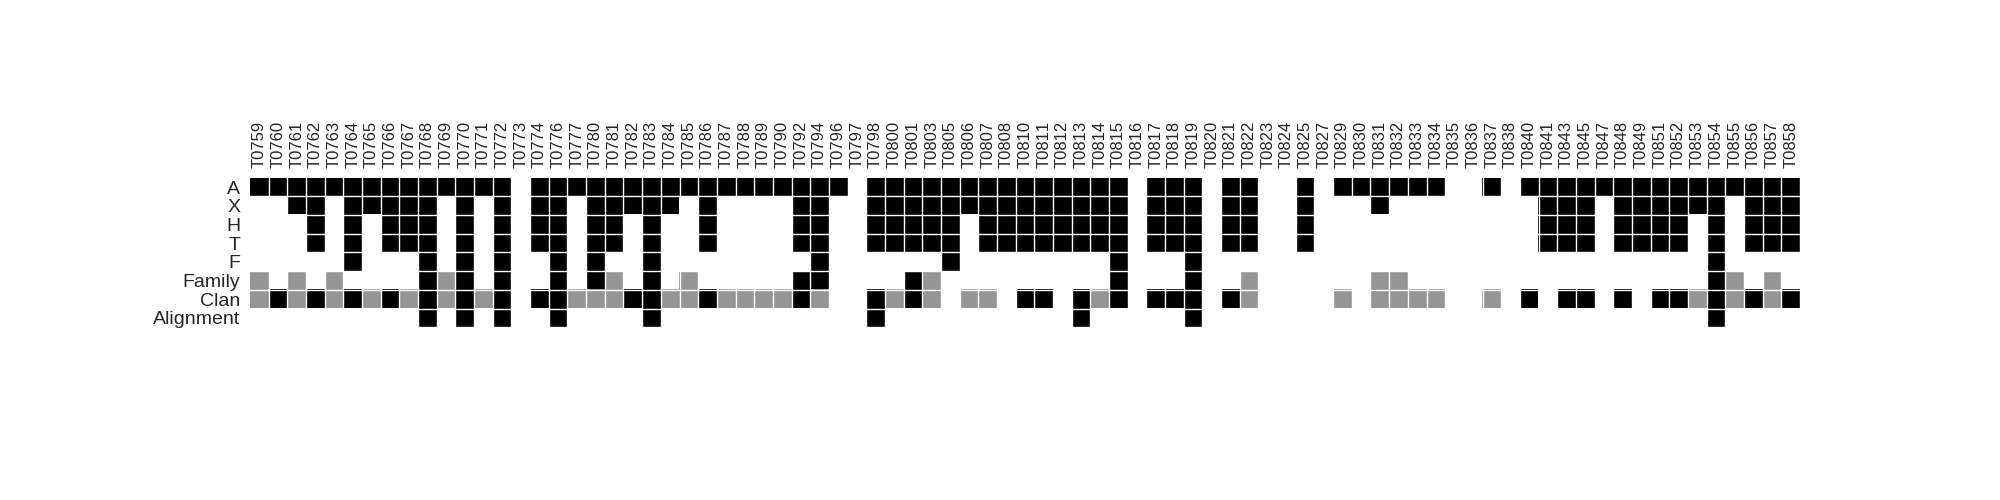
\includegraphics[width=\paperwidth]{Fig/summary_table.eps}
    }
%
    \caption{Overlap of the training set on each target domain of the
    test set (from T0759 to T0858). The first 5 rows of tiles
    correspond to the ECOD classification of protein domains (A-, X-,
    H-, T-, and F-groups). A black tile in any of these rows indicates
    that at least one structure from the training set belongs to the
    same ECOD group as the target. A white tile indicates that no
    structure belongs to the same group. Targets for which no ECOD
    classification is available are left empty (grey).
%%% GL: I see that all targets excluded from the analysis have an
%%% empty row of squares. Is T0838 excluded as well? What about the
%%% targets that are not in the list? (775, 778, 779, 791, 793, 795,
%%% 799, 802, 804, 809, 826, 828, 839, 842, 844, 846, 850) Were they
%%% all excluded from the CASP competition? The CASP11 QA paper
%%% mentions that the following targets were cancelled by the
%%% organizers: 778, 779, 791, 809, 842, 844, 846, 850. What about the
%%% other ones?
    A black tile in the ``Family'' row indicates that at least one
    structure from the training set belongs to the same Pfam family as
    the target. (Grey indicates that no Pfam family information is
    available for the target.) The ``Clan'' row shows similar
    information for Pfam clans. A black tile in the ``Alignment'' row
    indicates that at least one sequence in the training set aligns to
    the target sequence with an E-value smaller than $10^{-4}$. (Grey
    indicates that the protein structure is absent from the PDB database)}
%%% GL: You're using the code black=yes, white=no, grey=NA. I've
%%% modified the caption to reflect that.
%G: In case of alignment I skipped absent pdb structures(because I took sequences directly from structures, they are ususally shorter,
%than the sequences for predictions)
    \label{Fig:summaryTable}
\end{figure}



\subsection{Input}
The protein structure is represented as the density maps of eleven atom types. 
We used the types shown in the Table \ref{Tbl:atomTypes}. Initially 21 atom types were proposed by X.Zou et al. 
\cite{huang2006iterative, huang2008iterative} using SYBYL rule set \cite{wang2006automatic}. In this work we clustered similar
types due to the hardware constraints. The density of an atom was modeled using the function: 
$$
\rho(r) =  \begin{cases}
               e^{-\frac{r^2}{2}}&r\leq 2.0\AA~\\
               0                 &r>2.0\AA~\\
            \end{cases}
$$
Each atom density was projected to the grid for the corresponding atom type. The resolution of the grid was set to 1\AA~ and the size of 
each grid to 120x120x120 cells.

\begin{table}[H]
\begin{center}
\begin{tabular}{ c | l | l }
    
    Type & Description & Atoms \\
    \hline
    1 & Sulfur containing atoms & CYSSG, METSD, MSESE \\ \hline
    2 & Amide nitrogens & ASNND2, GLNNE2, backbone N \\ \hline
    3 & Aromatic nitrogens & HISND1, HISNE2, TRPNE1 \\ \hline
    4 & Guanidine nitrogens & ARGNH1, ARGNH2, ARGNE \\ \hline
    5 & Nitrogen with three hydrogens & LYSNZ \\ \hline
    6 & Carboxyl oxygen & ACEO, ASNOD1, GLNOE1, backbone O \\ \hline
    7 & Oxygen in hydroxyl group & SEROG, THROG1, TYROH \\ \hline
    8 & Oxygen in carboxyl group and terminus oxygen & ASPOD1, ASPOD2, GLUOE1, GLUOE2, \\
     & &  O-terminal, OT2-terminal, OXT-terminal \\ \hline
    9 & Sp2 carbon & ARGCZ, ASPCG, GLUCD, ACEC, \\
     & & ASNCG, GLNCD, backbone C \\ \hline
    10 & Aromatic carbon & HISCD2, HISCE1, HISCG, PHECD1 \\
     & & PHECD2, PHECE1, PHECE2, PHECG \\ 
     & & PHECZ, TRPCD1, TRPCD2, TRPCE2 \\
     & & TRPCE3, TRPCG, TRPCH2, TRPCZ2 \\
     & & TRPCZ3, TYRCD1, TYRCD2, TYRCE1 \\
     & & TYRCE2, TYRCG, TYRCZ \\ \hline
    11 & Sp3 carbon & ALACB, ARGCB, ARGCG, ARGCD \\
     & & ASNCB, ASPCB, GLNCB, GLNCG \\
     & & GLUCB, GLUCG, HISCB, HISCB \\
     & & ILECB, ILECD1, ILECG1, ILECG2 \\
     & & LEUCB, LEUCD1, LEUCD2, LEUCG \\
     & & LYSCB, LYSCD, LYSCG, LYSCE \\
     & & METCB, METCE, METCG, MSECB \\
     & & MSECE, MSECG, PHECB, PROCB \\
     & & PROCG, PROCD, SERCB, THRCG2 \\
     & & TRPCB, TYRCB, VALCB, VALCG1 \\
     & & VALCG2, ACECH3, THRCB, CYSCB \\
     & & backbone CA \\ \hline
    
\end{tabular}
    
    \caption {Atom types used in this work. In the atom notation the first three letters are the name of an aminoacid and the rest is 
    the atom name in the PDB format.}
    \label{Tbl:atomTypes}
\end{center}
\end{table}
Figure \ref{Fig:atomic_densities} shows an example of atomic densities of a peptide with the PDB code 5eh6.
Only non-zero densities are shown.

\begin{figure}[H]
    \centering
    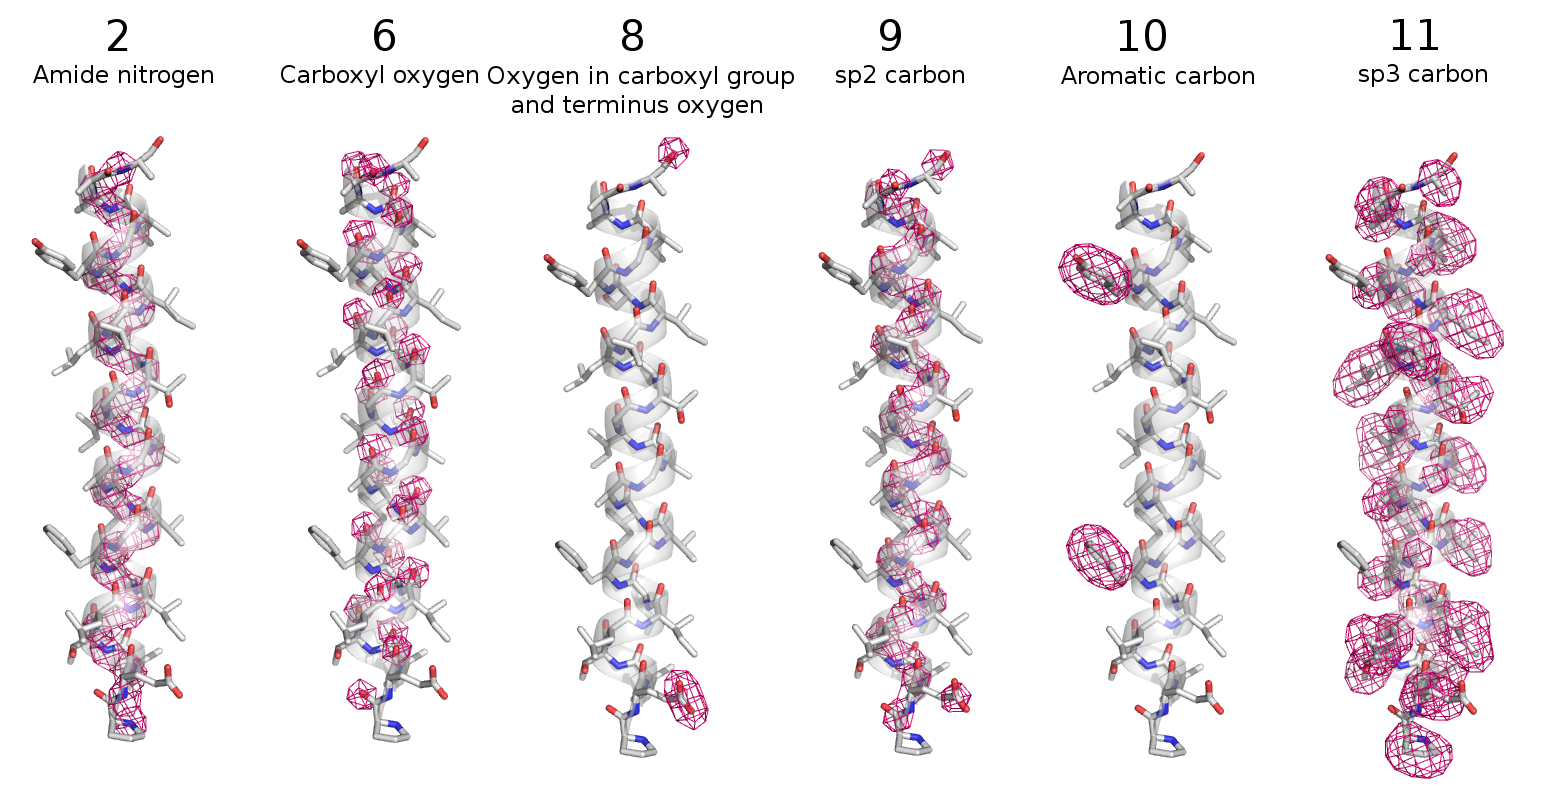
\includegraphics[width=\linewidth]{Fig/atomic_densities_V3.png}
    \caption{The example of the representation of a protein using atomic densities. The density map is 
    shown using the volumetric rendering plugin for PyMol. The pdb-code of the protein used for this visualization is 5eh6.
    The isosurface level was set to $0.5$.}
    \label{Fig:atomic_densities}
\end{figure}

\subsection{Model}
Convolutional neural networks were first proposed for the image recognition by Y.LeCun \cite{lecun1989backpropagation}, 
but gained recognition after the 
ImageNet 2012 competition \cite{krizhevsky2012imagenet}. 
In this work we use 3D convolutional networks to score protein structures. The network consists of 
basic layers that transform the input.
The schematic representation of the model architecture is shown on the Fig \ref{Fig:CNNModel}.
It is comprised of three blocks of alternating convolutional, 
volumetric batch normalization and ReLU layers and three 
fully connected layers with ReLU nonlinearities. The final output of the network is a single number, 
that is interpreted as a score of an input structure. Further we provide a consize description of each layer.

\begin{figure}[H]
    \centering
    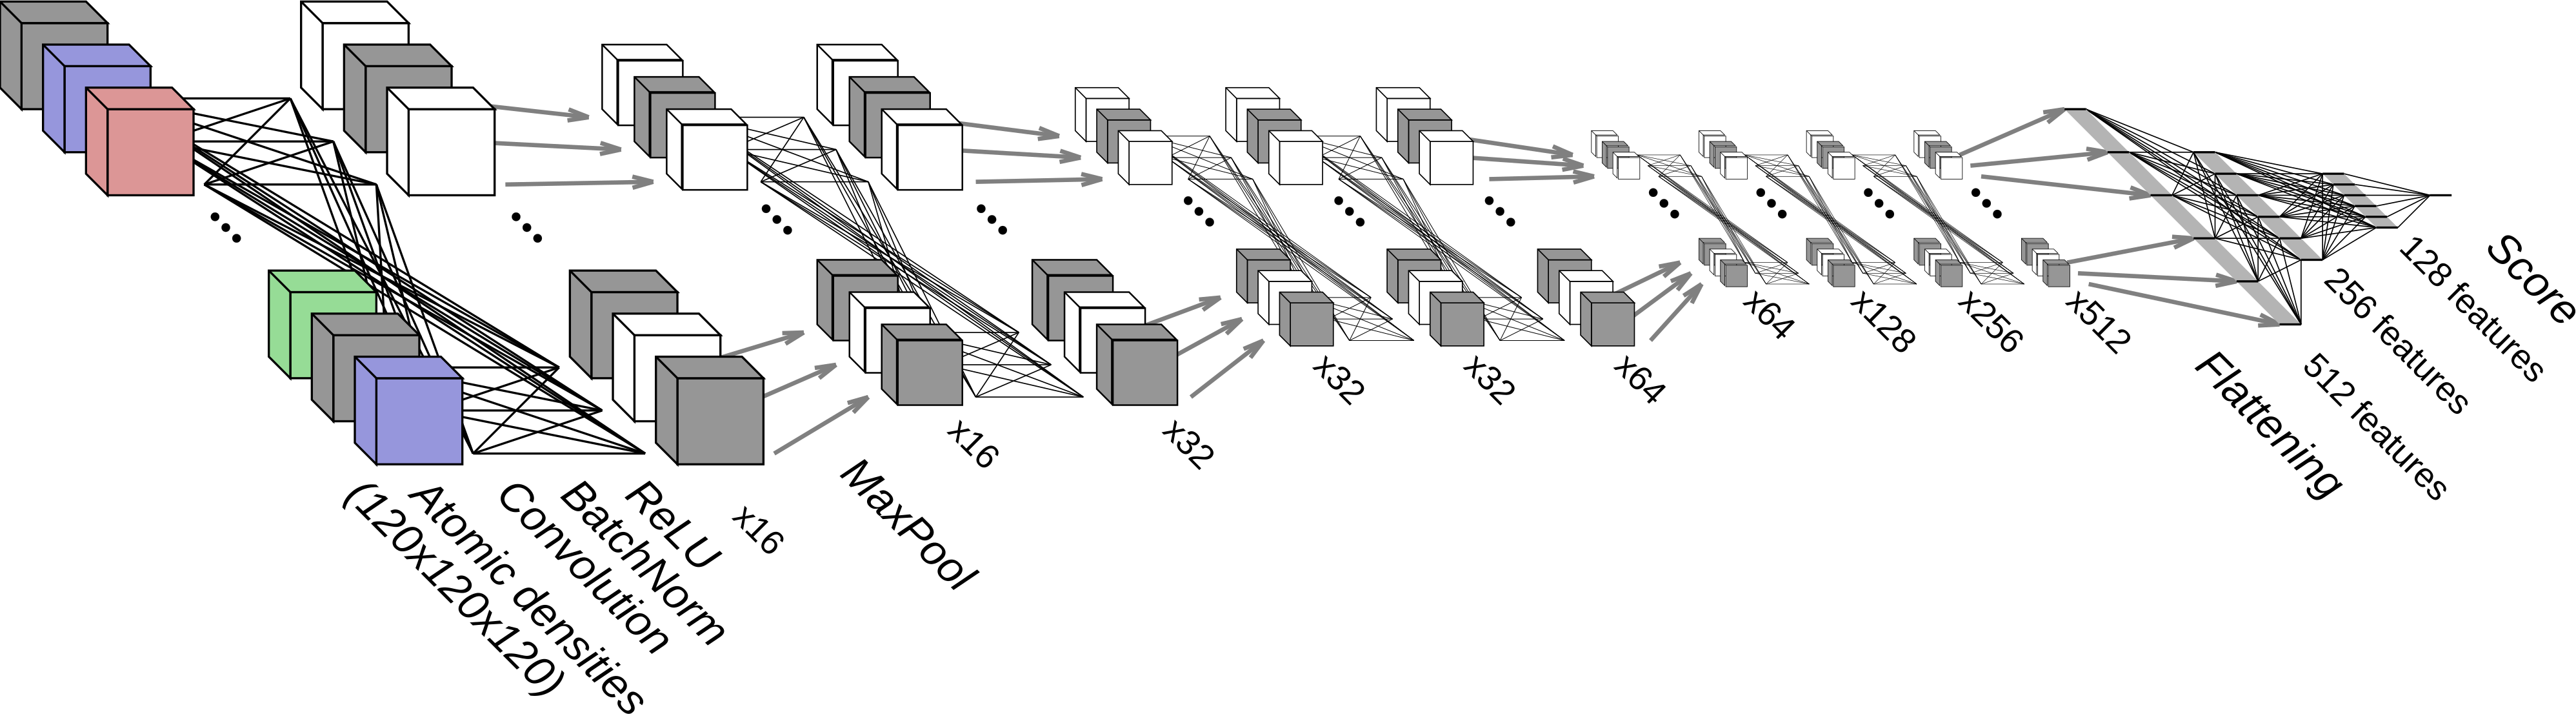
\includegraphics[width=\linewidth]{Fig/ConvnetDiagramV1.png}
    \caption{The schematic representation of the convolutional neural network architecture used in this work. 
    The arrows between the boxes denote maximum pooling layers and the connections denote 
    consequent 3d convolutional, batch normalization and ReLU layers. The numbers xM denote the number of filters 
    used in the corresponding 3d convolutional layer. The size of all filters and 
    maximum pooling domains are 3x3x3. The grey stripes denote one-dimensional vectors and crossed lines between them 
    stand for fully-connected layer with ReLU non-linearities. The details of the model parameters can be found in 
    Supplementary Information.}
    \label{Fig:CNNModel}
\end{figure}

The 3D convolutional layer takes $N$ input density maps and transforms them using $M$ filters
according to the following formula:
$$
f^{out}_i (\mathbf{r}) = \sum^{N}_{j=1} \int F_i (\mathbf{r} - \mathbf{\tau}) \cdot f^{in}_j(\mathbf{\tau}) ~d\tau, i \in [1,M]
$$
where filters are denoted using $F_j$. In standard implementations convolutions are approximated by the sum on a grid.
The ReLU nonlinearity is computed in the following way:
$$
f^{out}_i (\mathbf{r}) = \begin{cases}
               f^{in}_i(\mathbf{r})& f^{in}_i(\mathbf{r})\geq 0\\
               0                 &f^{in}_i(\mathbf{r})<0\\
            \end{cases}, i \in [1,M]
$$
The batch normalization layer was introduced by S.Ioffe and C.Szegedy \cite{ioffe2015batch} to address the problem of internal convariate shift:
the change in the distribution of subnetwork outputs due to the change in its parameters during the training. In practice, this layer takes the 
input and normalizes its values according to the mean values and variances of the corresponding values in the subset of examples used to estimate 
the gradient (minibatch):
$$
    \hat{f}^{in}_i(\mathbf{r}) = \frac{f^{in}(\mathbf{r}) - \mu_{B}}{\sqrt{\sigma^{2}_{B} + \epsilon}}, i \in [1,N_B]
$$
where $\mu_B(\mathbf{r}) = \frac{1}{N_B} \sum_{i=1}^{N_B} f^{in}_i(\mathbf{r})$ and 
$\sigma^{2}_{B} = \frac{1}{N_B} \sum_{i=1}^{N_B} \left( f^{in}_i(\mathbf{r}) - \mu_B (\mathbf{r}) \right)$. 
The constant $\epsilon$ is added to avoid division by zero, the number of 
examples in the minibatch is denoted as $N_B$. Afterwards, the output of this layer is computed by scaling the normalized inputs:
$$
f^{out}_i(\mathbf{r}) = \gamma \hat{f}^{in}_i(\mathbf{r}) + \beta, i \in [1,N_B]
$$
The parameters $\gamma$ and $\beta$ are learned along with other parameters of the network during the training.

The maximum pooling layer (MaxPool) is used to build a coarse-grained representation of the input. The output of this layer is 
the maximum over the cubes of the size $d$, that cover the input domain without overlapping. 
The output data domain is then $d$ times smaller than the input data box.

During the coarse-graining procedures the size of the input data box eventually shrinks to a single cell. The flattening layer reshapes the array of 
3d density maps to a single vector.

Afterwards, we compute several transformations using fully-connected layers. These layers transform a vector $\mathbf{x_{in}}$ in the follosing way:
$$
x_{out} = \mathbf{W} \cdot x + \mathbf{b}
$$
where $\mathbf{W}$ is a matrix and $\mathbf{b}$ is a vector, that are learned during the training.


\subsection{Loss functions}
We evaluated two scoring functions: linear regression and ranking scoring function. 
Let a decoy representation be denoted as $x_i$ and therefore the output
of the network on this decoy will be $f(x_i)$. Next, let $y_{ij}$ be the ordering coefficient of the two decoys we pick: 
$$
y_{ij} = \begin{cases}
               1& gdtts_i \leq gdtts_j \\
               -1& gdtts_i > gdtts_j \\
            \end{cases}
$$
Here $gdtts_i$ is the GDT-TS score of the $i$-th decoy. In principle, any target function can be chosen. 
The pairwise ranking scoring function has the following expression:

$$ L_{ij} = w_{ij} \cdot \max \left[ 0, 1 - y_{ij} \left( f \left( x_i \right) - f \left( x_j \right) \right) \right] $$

the term $w_{ij}$ represents an example weight:

$$
w_{ij} = \begin{cases}
               1& \left| gdtts_i - gdtts_j \right| > threshold \\
               0& otherwise \\ 
            \end{cases}
$$

where the $threshold$ is set to 0.1{\AA}. If the two decoys are too similar, 
we avoid scoring them against each other during the training, because it introduces 
the noise into the gradient and prevents optimization.


During the training procedure we load several decoys (batch) into memory and evaluate the model on them. 
Afterwards, we compute the average loss for the batch:
$$ L = \frac{1}{N} \sum_{i=1,j=1, i \neq j}^{M} L_ij $$ 
where $N$ is the number of pairs of decoys with the $w_{ij} > 0$ and $M$ is the number of decoys in a batch.

\subsection{Evaluation criteria}
We evaluated our algorithm using the correlation coefficients, Z-score and loss criterions. The correlation coefficents 
were computed between the score of 
our model and GDT-TS metric for all the decoys of each target protein in a test set and then averaged. 
The Z-score is the deviation of the score of 
the best decoy for a certain protein and average decoy score for this protein:
$$ 
Z-score = \frac{f( argmin(gdtts(x_i)) ) - <f(x)>}{std.dev.f(x)}
$$ 
the best decoy is the one with the lowest GDT-TS score. 
The loss criterion is the deviation of the GDT-TS of the best decoys for a protein from the GDT-TS score of the decoy with the lowest score:
$$ 
Loss = | max_i( gdtts_i ) - gdtts( argmin(f(x_i) ) |
$$ 

\subsection{Optimization and dataset sampling}
The optimization procedure of deep convolutional networks usually is stochastic: the function value and gradient 
is estimated on a small subset (batch) of all the training 
examples. We used the batch of size 10 due to the memory limitations. Afterward the parameters of the model are 
changed in the direction of the estimated gradient.
The parameter update step was performed using the Adam algorithm \cite{}. 

The dataset was sampled in the following way: first we chose a random protein from the dataset, then we sample decoys of this protein. 
The procedure is repeated for all the 
proteins in a dataset. One pass through all the proteins in a dataset is called epoch. 
The decoys are sampled in a homogeneous way: we divide all the decoys into $M$ clusters by the value of GDT-TS score. 
Precisely, the decoy $i$ belongs to the cluster  
number $ \left[ \frac{\max(gdtts) - gdtts_i}{\max(gdtts) - \min(gdtts)} \right] + 1$, where $\max(gdtts)$ and $\min(gdtts)$ 
are computed for all the decoys of 
the chosen protein. If there are empty clusters, then we take secon decoys from each non-empty and so on until we filled the batch. 
At the end of each epoch we randomly
shuffle the order of protein and the order of decoys in each cluster. 

Each decoy from the selected batch is randomly rotated and translated. The rotations are sampled uniformly \cite{}. The translation are chosen
in such a way, that the bounding box of the translated protein lies within the box of the size 120x120x120\AA. 

To select the final model we randomly divided the training set into training and validation subsets. The validation subset consists of 
35 targets and their decoys. This subset was not sampled during the training. 
Figure \ref{Fig:TrainingLoss} shows the Kendal tau, Pearsor R coefficients and the loss on the vaidation subset. 
The final model was chosen according to the minimum loss (epoch 40).
\begin{figure}[H]
    \centering
    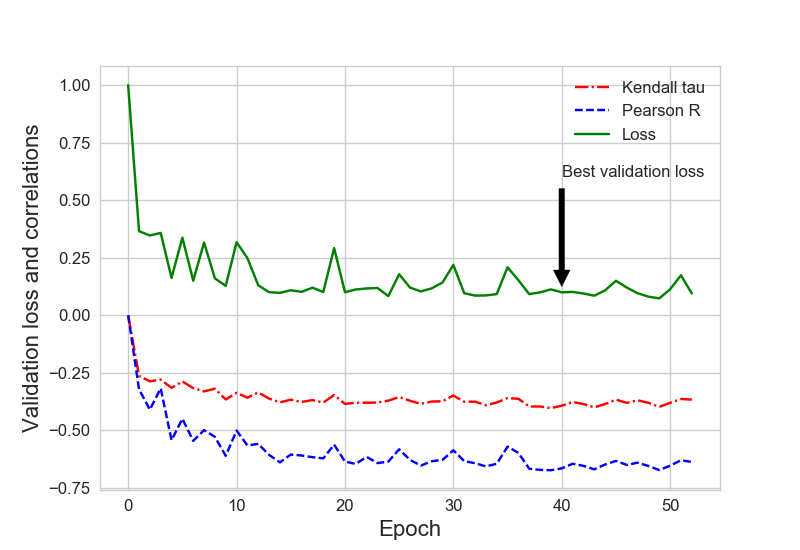
\includegraphics[width=\linewidth]{Fig/kendall_validation.png}
    \caption{The loss, Kendal tau and Pearson R coefficients evaluated on the validation subset during the training procedure. The epoch 
    denotes that all the targets in the training subset were sampled.}
    \label{Fig:TrainingLoss}
\end{figure}

The table \ref{Tbl:TrainingResults} summarizes the performance metrics on the training and validation sets for the model at epoch 40.

\begin{table}[H]
\begin{center}
\begin{tabular}{ c | c | c | c | c }
    Data subset & Loss & Pearson & Spearmann & Kendall \\
    \hline
    Training set     &0.146 &0.71 &0.61 &0.45 \\
    Validation set   &0.135 &0.71 &0.59 &0.44 \\ \hline

\end{tabular}
  \caption {Results of the model from epoch 40 on the training and validation subsets.}
    \label{Tbl:TrainingResults}
\end{center}
\end{table}

\section{Results}
During the training of the model we randomly sampled rotational and translational degrees of freedom of a decoy structure. Ideally, we 
want the score assigned by the model to a decoy to be invariant under these transformations. However Fig \ref{Fig:ScoreDistribution} 
shows that the distribution
of scores under rotations and translations follows the gaussian distribution. Therefore, to approximate the average score of a decoy we 
sample a score under random translation and rotation 20 times for each decoy in the test set. The final score is then the average of these 
samples.

\begin{figure}[H]
    \centering
    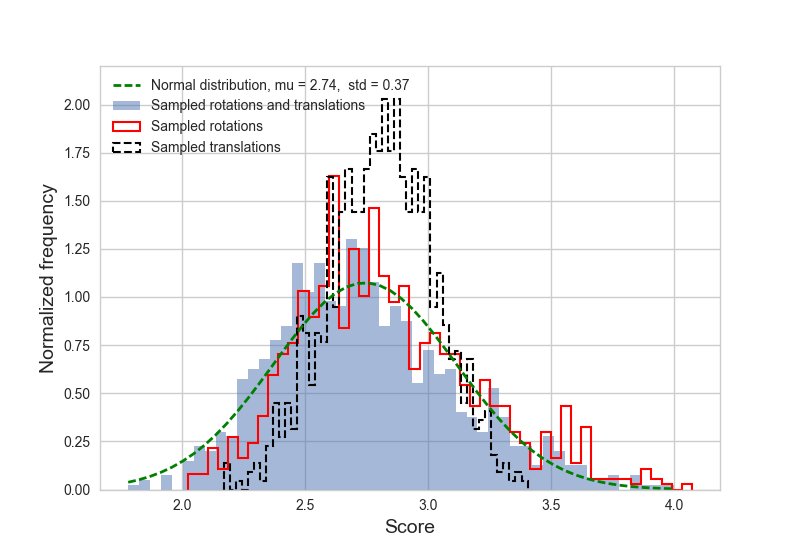
\includegraphics[width=\linewidth]{Fig/sampling_dist.png}
    \caption{The distribution of scores under random translations and rotations of the decoy LOOPP\_TS1 for the target T0342. The distributions 
    os scores under rotations only and translations only are shown with the dashed and solid lines respectively.
    The normal distribution fitted into the sampled scores under both rotations and translations is show with the dashed line. 
    The parameters of the normal distribution are: the average $\mu = 1.38$ and the standard deviation $\sigma = 0.42$.}
    \label{Fig:ScoreDistribution}
\end{figure}


Table \ref{Tbl:TestResults} shows the comparisson of our model with the state of art methods used for the decoy quality assessement. 
To evaluate the performance we used CASP11 stages 1 and 2 datasets. 
These datasets were preprocessed using SCWRL program to optimize side-chains. 

\begin{table}[H]
\begin{center}
\begin{tabular}{ c | c | c | c | c }
    \multicolumn{5}{ c }{Stage 1} \\ \hline

    QA method & Loss & Pearson & Spearmann & Kendall \\
    \hline
    ProQ2   &0.090 &0.643 &0.506 &0.379 \\
    Qprob   &0.097 &0.631 &0.517 &0.389 \\
    \textbf{3DCNN}   &\textbf{0.072} &0.530 &0.415 &0.318 \\
    RWplus  &0.135 &0.536 &0.433 &0.433 \\ \hline
    
    \multicolumn{5}{ c }{Stage 2} \\ \hline
    
    ProQ2   &\textbf{0.058} &0.372 &0.366 &0.256 \\ 
    Qprob   &0.068 &0.381 &0.387 &0.272 \\
    \textbf{3DCNN}     &\textbf{0.064} &\textbf{0.415} &\textbf{0.402} &\textbf{0.283} \\
    RWplus  &0.084 &0.295 &0.314 &0.220 \\ \hline

\end{tabular}
    
    \caption {Results of our method(3DCNN) and the other state-of-art quality assessment programs on the CASP11 dataset Stage 1 and 2.
            Table shows the absolute average values of correlation coefficients. The averaging was performed for each target in the 
            dataset. Afterwards all the values were averaged over all the targets.}
    \label{Tbl:TestResults}
\end{center}
\end{table}

\section{Analysis}


\section{Discussion}

\bibliography{citations.bib}{}
\bibliographystyle{plain}


\end{document}
